\documentclass{article}

% --- PACKAGES ---
\usepackage[utf8]{inputenc}
\usepackage[T1]{fontenc}
\usepackage[margin=1in]{geometry} 
\usepackage{amsmath}               
\usepackage{graphicx}              
\usepackage{booktabs}              
\usepackage{listings}              
\usepackage{xcolor}                
\usepackage{hyperref}              
\usepackage{caption}               
\usepackage{float}                 
\usepackage{gvv}
\usepackage{gvv-book} 

\lstdefinestyle{pythonstyle}{
    language=Python,
    backgroundcolor=\color{gray!10},
    commentstyle=\color{green!60!black},
    keywordstyle=\color{blue},
    stringstyle=\color{red!60!black},
    basicstyle=\ttfamily\footnotesize,
    breakatwhitespace=false,
    breaklines=true,
    captionpos=b,
    keepspaces=true,
    numbers=left,
    numbersep=5pt,
    showspaces=false,
    showstringspaces=false,
    showtabs=false,
    tabsize=2,
    morekeywords={plt, np, LA} 
}

\lstdefinestyle{arduinostyle}{
    language=C++,
    backgroundcolor=\color{gray!10},
    commentstyle=\color{green!60!black},
    keywordstyle=\color{blue},
    stringstyle=\color{red!60!black},
    basicstyle=\ttfamily\footnotesize,
    breakatwhitespace=false,
    breaklines=true,
    captionpos=b,
    keepspaces=true,
    numbers=left,
    numbersep=5pt,
    showspaces=false,
    showstringspaces=false,
    showtabs=false,
    tabsize=2,
    morekeywords={LiquidCrystal, pinMode, analogRead, digitalWrite, Serial, HIGH, LOW, INPUT_PULLUP, OUTPUT} 
}

% --- TITLE INFORMATION ---
\title{HARDWARE PROJECT EE-1030 \\ DIGITAL THERMOMETER}
\author{KARTIK LAHOTI - EE 25 BTECH11032 \\ SUBHODEEP CHAKRABORTHY - EE 25 BTECH11OSS}
\date{31st October 2025}

% --- BEGIN DOCUMENT ---
\begin{document}

\maketitle
\tableofcontents
\newpage

\section*{OBJECTIVE}
To design, implement and validate a digital thermometer, using a PT-100 Resistance Temperature Detector (RTD) for measurement, an Arduino microcontroller for processing and a 16x2 LCD for output.

This experiment uses the least squares approach to estimate a model for ambient temperature versus voltage.

\section*{THEORY}
Resistance of a PT-100 varies with temperature as given by the Callendar-Van Dusen Equation:
\begin{align}
    R(T) = R_0(1 + A \times T + B \times T^2)
\end{align} 
Values of A and B can be found experimentally. When placed in a voltage divider circuit, the voltage across the PT-100 can be measured and used to infer temperature as per the above relationship.

\section*{APPARATUS}
\begin{enumerate}
    \item Arduino UNO
    \item PT-100 RTD
    \item Lab-grade Thermometer
    \item Electric Kettle
    \item Jumper cables
    \item Breadboard
    \item Android Phone
    \item Resistors of at most 5\% tolerance (130$\Omega$ used)
    \item Push Button
    \item Potentiometer
    \item 16x2 LCD
    \item JST XH 2-pin wire connector
    \item Arduino Cable
    \item USB-A to USB-C convertor
\end{enumerate}

\section*{CIRCUIT REPRESENTATION}
\begin{figure}[H]
    \centering
    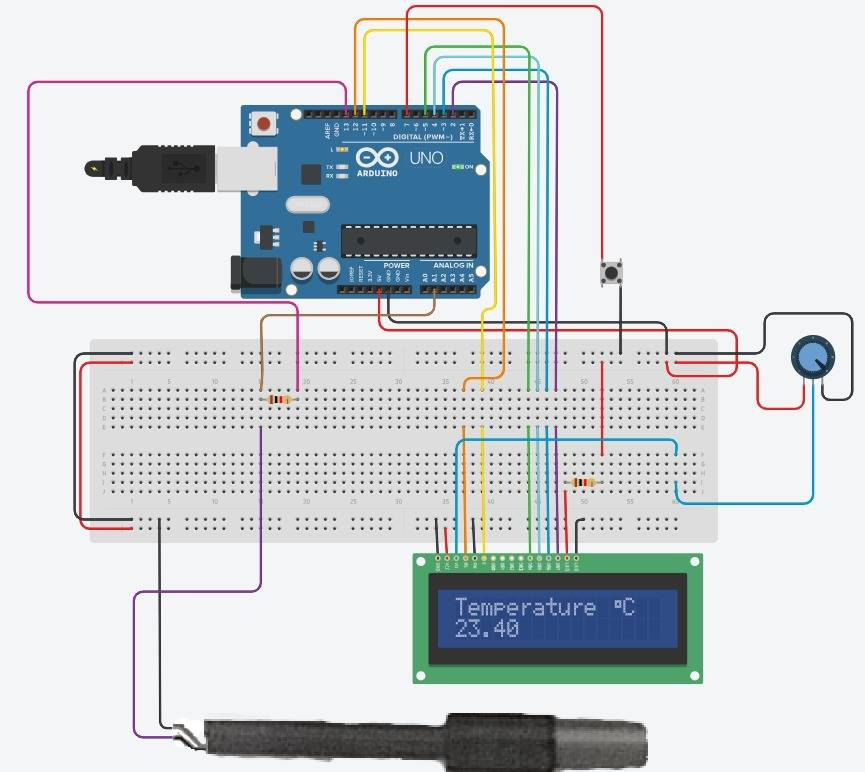
\includegraphics[width=0.9\columnwidth]{figs/circuit_schematic.jpg}
    \caption{Circuit Schematic}
    \label{fig:schematic}
\end{figure}

\newpage
\section{PROCEDURE}

\subsection{Circuit Assembly}
Make connections as per the circuit schematic. Note that while the push button in the schematic has 4 terminals, same connections are applicable for 2-terminal push-buttons.
Ensure that a resistor of appropriate denomination is connected to the LED backlight of the LCD.

To choose the value of the resistor in series with the PT-100, our aim was to maximize the sensitivity of the variation of voltage across the PT-100 with temperature.
Taking $V$ as the voltage source, $R$ as value of resistance of PT-100, $x$ as resistance in series, we have voltage across PT-100 as:
\begin{align} V_{R} = V \frac{R}{x+R} \end{align}
    
Sensitivity $(S) = \frac{dV_R}{dR}$. Using the quotient rule:
\begin{align} S = \frac{d}{dR} \left[ V \frac{R}{x+R} \right] = V \left[ \frac{(1)(x+R) - R(1)}{(x+R)^2} \right] = \frac{Vx}{(x+R)^2} \end{align}
To maximise sensitivity with respect to the series resistor $x$, we set $\frac{dS}{dx} = 0$:
\begin{align} \frac{dS}{dx} = \frac{d}{dx} \left[ V \frac{x}{(x+R)^2} \right] = V \left[ \frac{(1)(x+R)^2 - x(2(x+R))}{(x+R)^4} \right] = 0\end{align}
\begin{align} V \left[ \frac{(x+R) - 2x}{(x+R)^3} \right] = 0 \end{align}
\begin{align}V \frac{R-x}{(x+R)^3} = 0 \end{align}
\begin{align} \Rightarrow x=R \end{align}
Since $R$ varies with temperature, we take value of $x$ as the median of $R$'s expected range, i.e.; $x = 130 \Omega$.

\subsection{Platformio Setup}
In order to work with the Arduino on an Android phone, we need to setup platformio and Arduino Droid on Termux.

\subsubsection{Platformio}
\begin{enumerate}
    \item Login to \texttt{proot-distro}.
    \item Download and run the platformio installer.
    \begin{lstlisting}[language=Bash]
wget -O get-platformio.py https://raw.githubusercontent.com/platformio/platformio-core-installer/master/get-platformio.py
python3 get-platformio.py
    \end{lstlisting}
    \item Follow on-screen steps to install pio to PATH, if necessary.
    \item Create a folder \texttt{PT100} in \texttt{/sdcard} path and initialize the project.
    \begin{lstlisting}[language=Bash]
mkdir PT100
pio project init --board uno --ide vscode --project-dir PT100
    \end{lstlisting}
    \item Add code in \texttt{src/main.cpp} in project folder.
    \begin{lstlisting}[language=Bash]
nvim PT100/src/main.cpp
    \end{lstlisting}
    \item Compile file.
    \begin{lstlisting}[language=Bash]
pio run
    \end{lstlisting}
\end{enumerate}

\subsubsection{Arduino Droid}
\begin{enumerate}
    \item Install the \href{https://apkpure.com}{Apkpure} app on device.
    \item Install Arduino Droid version 6.3.0 from the Apkpure app (newer versions do not work reliably on recent Android versions).
    \item In Arduino Droid, click : \textgreater{} Actions \textgreater{} Upload \textgreater{} Upload precompiled.
    \item Navigate to project folder and upload \texttt{.pio/build/uno/firmware.hex} with Arduino connected.
\end{enumerate}

\subsection{Taking Readings}
Dip both PT-100 and thermometer into kettle. Power on the devices and take readings of voltage-temperature mappings for different temperatures using the kettle.

\subsection{Training of Model}
Using the collected data, apply least squares as per the Python code.

\subsection{Validation of Results}
Take another set of readings and map for temperature versus temperature. Use the Python code to generate error plot.

\subsection{Error Analysis}
This implementation results in the following measures of error:
\begin{enumerate}
    \item Mean: 1.358$^{\degree}$C
    \item Median: 1.595$^{\degree}$C
    \item Mode: 1.81$^{\degree}$C
\end{enumerate}
    
\subsection{Observations}
LCD could display expected values. Potentiometer could adjust contrast. Push button switched between $^{\degree}$C and $^{\degree}$F reliably. Button could also switch to display voltage reading on LCD correctly.

\newpage
\section{CALIBRATION MODEL}
The collected data consists of values of voltage $V$ across the PT-100 for temperature $T$ over a large range of known temperatures. In this data, we know that maximum error is present in the values of $V$, and the goal is to find a predictive model for $T$ in terms of $V$.

Given this and the hardware-level computational constraints of the Arduino, the best modelling method that balances accuracy as well as computational complexity is the least squares method.

\subsection{Least Squares Method}
An empirical model for the data can be formed using least squares. The basic physical relation is given by the Callendar-Van Dusen equation:
\begin{align}
    R(T) = A + BT + CT^2
\end{align}  
The above expression which gives the resistance of pt-100 sensor at a temperature $T$, can be used to find voltage across pt-100 in the voltage divider circuit used.
\begin{align}
    V_{Pt-100} = \frac{R(T) \times V_s}{R_s + R(T)} 
\end{align}  
where $V_s$ ($5$V) is source voltage, $R_s$ ($130\Omega$) is resistance in series.

Analysing the graph of $V_{PT-100}$ in the relevant temperature range, we see that it approximates to a parabola.
\begin{align}
    V_{PT-100} = \alpha + \beta T + \gamma T^2
    \label{eq:V_of_T}
\end{align}
Since the greater amount of errors is in the measurements of $V$, normally applying least squares on Equation (\ref{eq:V_of_T}) would be preferred.
However, since the intention is to build a predictive model for $T$, the better choice is applying least squares on equation (\ref{eq:T_of_V}):
\begin{align}
    T(V) = \eta_0 + \eta_1 V + \eta_2 V^2
    \label{eq:T_of_V}
\end{align}
where $V$ is voltage across pt-100.
Equation (\ref{eq:V_of_T}) and Equation (\ref{eq:T_of_V}) are equivalent in our operating range since a quadratic $y = pu^2 + qu + r$ can be approximated by a quadratic for a small region as $u = ly^2 + my + n$.

\subsection{In Matrix Form}
The system $ \vec{T} = \vec{V} \vec{\eta} $ is expressed as:

\begin{align}
    \myvec{T1 \\ T2 \\ \vdots \\ T_n } = \myvec{1 & V_1 & V_1^2 \\
    1 & V_2 & V_2^2 \\
    \vdots & \vdots & \vdots \\
    1 & V_n & V_n^2} \myvec{ \eta_0 \\ \eta_1 \\ \eta_2}
\end{align}

Goal: To find best-fit $\vec{\eta}$ for the equation.
Since $\vec{V}$ is a tall matrix for our data, this system of equation is overdetermined and usually has no exact solution.

We try to find ${\vec{\eta}}$ that minimizes $\norm{\vec{V}\vec{\eta} - \vec{T}}$ , i.e., the vector in $\text{Col}(\vec{V})$ closest to $\vec{T}$ in Euclidean distance.
Using the normal equations for least squares, we estimate $\hat{\mathbf{\eta}}$:
\begin{align}
    \vec{\eta} = \brak{\vec{V}^{\top}\vec{V}}^{-1}\vec{V}^{\top}\vec{T}
\end{align}
After running the obtained data through the python code, the trained model is obtained giving best-fit $\vec{\eta}$ as:
\begin{align}    
\vec{\eta} = 
\myvec{
    -367.48044857 \\
    37.67235012 \\
    54.77146835
}\end{align}
This least square solution is obtained from the formula on Python Code Line 30.
When the least square solution was found using \texttt{np.linalg.lstsq} (line 33) and using SVD (lines 37-38), the $\hat{\mathbf{\eta}}$ vector obtained was equal:
\begin{align}
    \vec{\eta} = \myvec{-367.48044858 \\
    37.67235009 \\
    54.77146835}
\end{align}

Even though the \texttt{linalg} module of numpy has a \texttt{lstsq} function, internally it computes the solution using Singular Value Decomposition (SVD) for improved numerical stability and accuracy.

\section{Training Data}
\begin{table}[H]
    \centering
    \caption{Training Data}
    \begin{tabular}{cc}
        \toprule
        Temperature ($^{\degree}$C) & Voltage Reading (V) \\
        \midrule
        $27.5$ & $2.3558$ \\
        $33.8$ & $2.3851$ \\
        $37.9$ & $2.3998$ \\
        $41.5$ & $2.4145$ \\
        $47.9$ & $2.4389$ \\
        $50.6$ & $2.4487$ \\
        $52.6$ & $2.4536$ \\
        $57.6$ & $2.4633$ \\
        $62.2$ & $2.4780$ \\
        $63.8$ & $2.4780$ \\
        $66.1$ & $2.4878$ \\
        $68.5$ & $2.4927$ \\
        $73.3$ & $2.5122$ \\
        $74.9$ & $2.5171$ \\
        $77.7$ & $2.5269$ \\
        $81.1$ & $2.5367$ \\
        $84.3$ & $2.5513$ \\
        $89.5$ & $2.5660$ \\
        $91.7$ & $2.5709$ \\
        $96.7$ & $2.5904$ \\
        $44.8$ & $2.4218$ \\
        $59.3$ & $2.4682$ \\
        $64.9$ & $2.4829$ \\
        $70.9$ & $2.5024$ \\
        $87.4$ & $2.5611$ \\
        \bottomrule
    \end{tabular}
    \label{tab:trainingdata}
\end{table}


\begin{figure}[H]
    \centering
    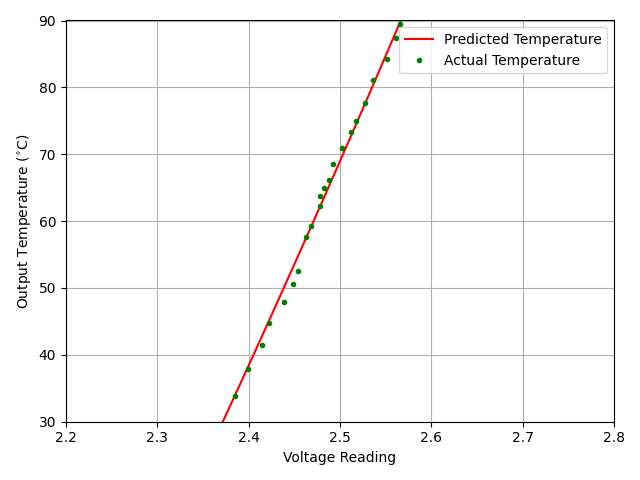
\includegraphics[width=0.8\columnwidth]{figs/train.png}
    \caption{Training Data Plot}
    \label{fig:trainplot}
\end{figure}

\newpage
\section{Validation Data}
\begin{table}[H]
    \centering
    \caption{Validation Data}
    \begin{tabular}{ccc}
        \toprule
        Predicted Temp ($^{\degree}$C) & True Temp ($^{\degree}$C) & Voltage Reading (V) \\
        \midrule
        $36.89$ & $36.1$ & $2.3949$ \\
        $42.78$ & $42.5$ & $2.4145$ \\
        $51.68$ & $50.3$ & $2.4438$ \\
        $59.18$ & $57.1$ & $2.4682$ \\
        $63.71$ & $61.9$ & $2.4829$ \\
        $71.31$ & $69.5$ & $2.5073$ \\
        \bottomrule
    \end{tabular}
    \label{tab:validationdata}
\end{table}


\begin{figure}[H]
    \centering
    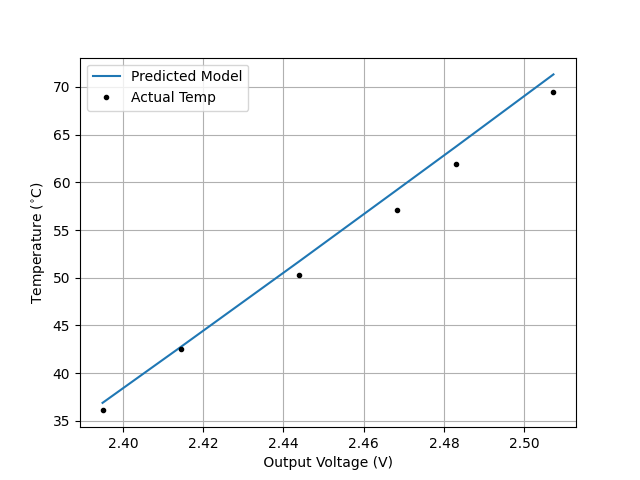
\includegraphics[width=0.8\columnwidth]{figs/valid.png}
    \caption{Validation Data Plot}
    \label{fig:validplot}
\end{figure}

\newpage
\section{PYTHON CODE}
\begin{lstlisting}[style=pythonstyle, caption={Python Code for Model Training and Validation}, label={lst:python}]
import numpy as np
import numpy.linalg as LA
import sys
from pathlib import Path
import matplotlib.pyplot as plt

# --- Load Training Data ---
data = {}
# Assumes 'training_data.txt' is in the same folder
with open(Path(__file__).resolve().parent / "training_data.txt") as fp:
    for line in fp:
        # Assuming format: "Temperature Voltage"
        parts = line.split()
        if len(parts) >= 2:
            data[parts[0]] = parts[1]

try:
    n = int(sys.argv[1]) # Polynomial degree
except IndexError:
    n = 2 # Default to quadratic

T = np.empty((len(data), 1))
V = np.empty((len(data), n + 1))
i = 0
for temp, volt in data.items():
    T[i] = float(temp)
    volts = []
    volt_val = float(volt)
    for j in range(n + 1):
        if j == 0:
            volts.append(1) # Column for eta_0
        else:
            volts.append(volts[-1] * volt_val)
    V[i] = volts
    i += 1

# --- Least Squares Solutions ---
# 1. Using Normal Equation
lst_squares = LA.inv(V.T @ V) @ V.T @ T
print("--- Solution from Normal Equation ---")
print(lst_squares)

# 2. Using numpy.linalg.lstsq (preferred)
lstsq_sol = np.linalg.lstsq(V, T, rcond=None)[0]
print("\n--- Solution from np.linalg.lstsq ---")
print(lstsq_sol)

# 3. Using SVD
U, S, VT = np.linalg.svd(V, full_matrices=False)
n_svd = VT.T @ np.linalg.inv(np.diag(S)) @ U.T @ T
print("\n--- Solution from SVD ---")
print(n_svd)

# --- Plot Code (Training) ---
plt.figure(1)
plt.plot(V[:, [1]], V @ lst_squares, color="red", label="Predicted Temperature")
plt.plot(V[:, [1]], T, 'k.', label="Actual Temperature")
plt.grid()
plt.xlim(2.2, 2.8)
plt.ylim(30, 90)
plt.ylabel('Output Temperature ($^{\degree}$C)')
plt.xlabel('Voltage Reading (V)')
plt.tight_layout()
plt.legend(loc='best')
plt.savefig(Path(__file__).resolve().parent / "train.png")
plt.close('all')

# --- Validation ---
valid_data = {}
# Assumes 'validation_data.txt' is in the same folder
# Format: "Predicted True Voltage"
with open(Path(__file__).resolve().parent / "validation_data.txt") as fp:
    for line in fp:
        parts = line.split()
        if len(parts) >= 3:
            # Key: True Temp, Value: [Voltage, Predicted Temp]
            valid_data[parts[1]] = [parts[2], parts[0]]

T_thermo = np.empty((len(valid_data), 1)) # True Temp
Vv = np.empty((len(valid_data), n + 1))
T_pt = np.empty((len(valid_data), 1))     # Predicted Temp (from model)
i = 0
for temp_true, volt_data in valid_data.items():
    T_thermo[i] = float(temp_true)
    T_pt[i] = float(volt_data[1]) # Predicted Temp from file
    volts = []
    volt_val = float(volt_data[0]) # Voltage from file
    for j in range(n + 1):
        if j == 0:
            volts.append(1)
        else:
            volts.append(volts[-1] * volt_val)
    Vv[i] = volts
    i += 1

# --- Plot Code (Validation) ---
plt.figure(2)
# Note: T_pt is the *predicted* temp from the file. 
# Vv @ lst_squares would be a *new* prediction.
# The plot from the doc plots T_pt vs V, and T_thermo vs V.
plt.plot(Vv[:, [1]], T_pt, 'r-', label="Predicted Model")
plt.plot(Vv[:, [1]], T_thermo, 'k.', label="Actual Temp")
plt.xlabel('Output Voltage (V)')
plt.ylabel('Temperature ($^{\degree}$C)')
plt.grid()
plt.legend(loc='best')
plt.savefig(Path(__file__).resolve().parent / "valid.png")
\end{lstlisting}

\newpage
\section{ARDUINO PROGRAM}
\begin{lstlisting}[style=arduinostyle, caption={Arduino Sketch (main.cpp)}, label={lst:arduino}]
#include <LiquidCrystal.h>

// Initialize the library with the numbers of the interface pins
// LiquidCrystal lcd(RS, E, D4, D5, D6, D7);
LiquidCrystal lcd(12, 11, 5, 4, 3, 2);

int status = 1; // Controls the display mode
int buttonPin = 7; // Push button on digital pin 7

// Custom char for degree symbol
byte degreeSymbol[8] = {
    0b00110,
    0b01001,
    0b01001,
    0b00110,
    0b00000,
    0b00000,
    0b00000,
    0b00000
};

void setup() {
    lcd.begin(16, 2);
    lcd.clear();
    Serial.begin(9600);
    
    // Using digital pin 13 as a stable 5V source (as per doc)
    pinMode(13, OUTPUT);
    digitalWrite(13, HIGH);

    // Button pin setup
    pinMode(buttonPin, INPUT_PULLUP); // Use internal pull-up resistor
    
    // Create the custom degree symbol
    lcd.createChar(0, degreeSymbol);
}

void loop() {
    float volt, temp, tempf;
    
    // These are the coefficients (eta_0, eta_1, eta_2) from Python
    float a0 = -367.48044857;
    float a1 = 37.67235012;
    float a2 = 54.77146835;

    // Read analog pin A1 (as per doc)
    volt = (5.0 * analogRead(A1) / 1023.0);

    // Check for button press
    if (digitalRead(buttonPin) == LOW) { // Button is pressed
        status++;
        if (status > 2) {
            status = 0; // Cycle through modes 0, 1, 2
        }
        delay(250); // Simple debounce
    }

    // Calculate temperature from voltage using the model
    temp = a0 + (a1 * volt) + (a2 * volt * volt);
    
    // Convert to Fahrenheit
    tempf = temp * 1.8 + 32.0;

    // Clear the LCD for new data
    lcd.clear(); 

    switch (status) {
        case 1: // Display Temperature in Celsius
            lcd.setCursor(0, 0);
            lcd.print("Temperature ");
            lcd.write((byte)0); // Print degree symbol
            lcd.print("C");
            lcd.setCursor(0, 1);
            lcd.print(temp);
            Serial.println(temp);
            break;
            
        case 2: // Display Temperature in Fahrenheit
            lcd.setCursor(0, 0);
            lcd.print("Temperature ");
            lcd.write((byte)0); // Print degree symbol
            lcd.print("F");
            lcd.setCursor(0, 1);
            lcd.print(tempf);
            Serial.println(tempf);
            break;
            
        default: // case 0: Display Voltage Reading
            lcd.setCursor(0, 0);
            lcd.print("Voltage Reading");
            lcd.setCursor(0, 1);
            lcd.print(volt, 4); // Print voltage with 4 decimal places
            Serial.println(volt, 4);
            break;
    }
    
    delay(200); // Refresh rate
}
\end{lstlisting}

\newpage
\section*{ARDUINO FUNCTIONS}
\begin{enumerate}
    \item Initialize LCD and analog input pin.
    \item Read analog voltage: $V = \text{analogRead}(\text{pin}) \times 5.0 / 1023.0$
    \item Compute temperature (In Celsius) using: $T_C = \eta_0 + \eta_1 V + \eta_2 V^2$
    \item Compute temperature (In Fahrenheit) using: $T_F = T_C \times 1.8 + 32.0$
    \item LCD can switch modes and display temperature both in Celsius and in Fahrenheit.
    \item Separate debugging mode showing current voltage reading across the sensor.
    \item Stateful push button logic to remember and switch between modes of operation.
\end{enumerate}

\section*{Learning Outcomes}
\begin{enumerate}
    \item Understanding PT-100 sensor characteristics and errors in sensor instrumentation.
    \item Designing and implementing a complete embedded system which interfaces an analog sensor with an Arduino microcontroller.
    \item Implementing least squares regression for different complexities and modeling approaches to solve for the best-fit polynomial model.
    \item Applying the industry-standard Callendar-Van Dusen equation to demonstrate fitting a physical model to a curve.
    \item Applied error minimisation for common issues:
    \begin{itemize}
        \item Separated sensor and LCD wiring to reduce confusion.
        \item Found high amounts of noise in Arduino 5V-pin, after testing decided to use the much more stable output of a digital pin as sensor power source.
    \end{itemize}
    \item Implemented advanced functionality like user-controlled mode switching.
\end{enumerate}

\section*{CONCLUSION}
This project successfully implemented a temperature sensor using an Android, Arduino microcontroller, PT-100 sensor, LCD and the least squares approach.

\end{document}
